\section{Computing Platforms for ADAS and AD}

\begin{wrapfigure}{r}{0.45\textwidth}
    \centering
    \vspace{-10pt}
    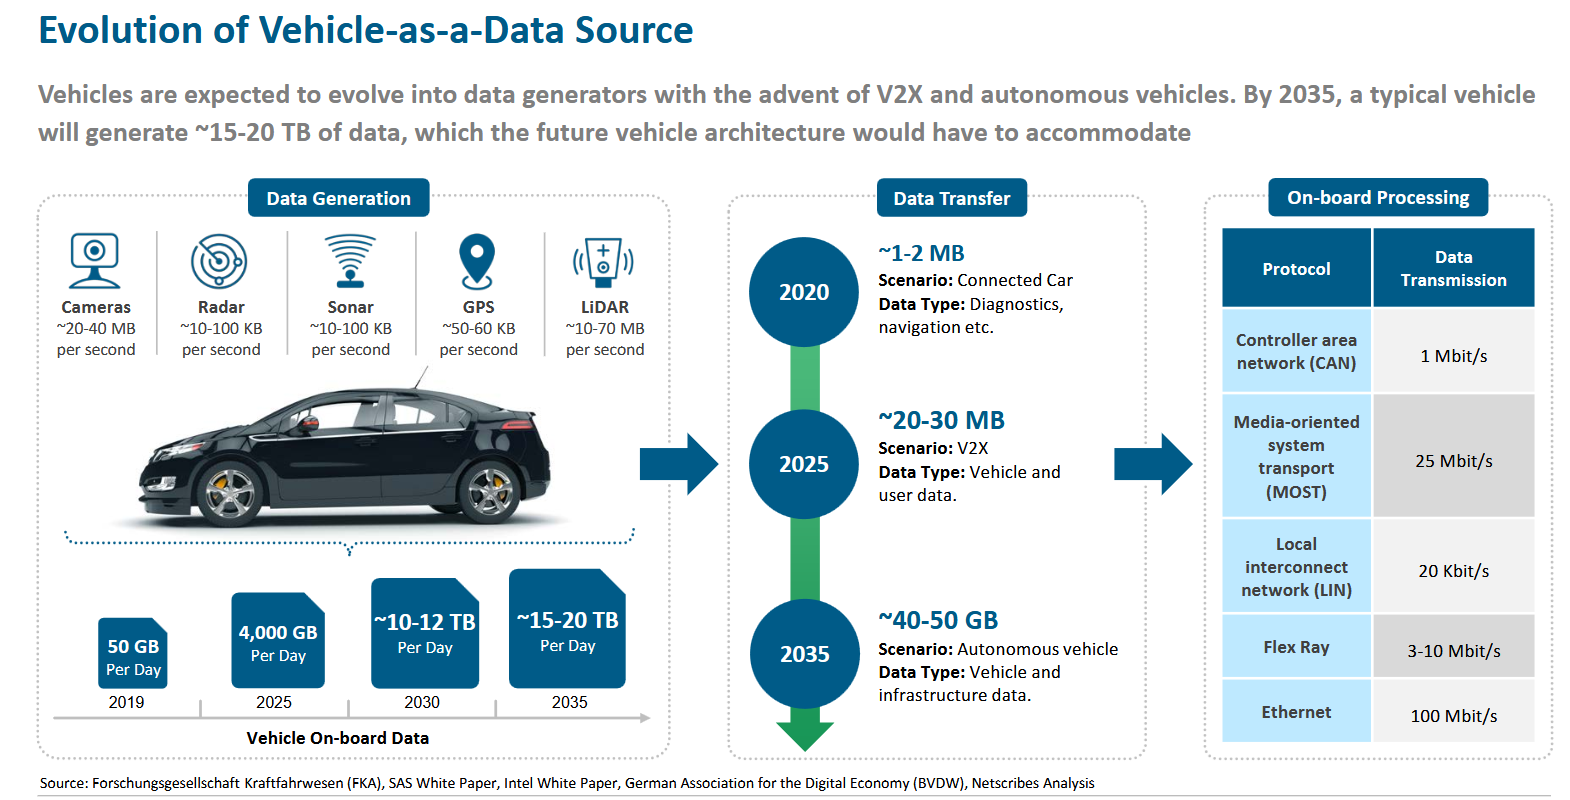
\includegraphics[width=\linewidth]{images/C2_1.png}
    \caption{Evolution of the vehicle as a data source}
    \vspace{-10pt}
\end{wrapfigure}
Modern vehicles are becoming real \textbf{data generators}, especially with the advent of V2X (Vehicle-to-Everything) communication and autonomous driving.
Every sensor produces a continuous stream of data:
\begin{compactitemize}
    \item \textbf{Cameras}: $\sim$20--40 MB per second;
    \item \textbf{LiDAR}: $\sim$10--70 MB per second;
    \item \textbf{Radar} and \textbf{Sonar}: $\sim$10--100 KB per second;
    \item \textbf{GPS}: $\sim$50 KB per second.
\end{compactitemize}

By 2035 a typical vehicle is expected to generate $\sim$\textbf{15--20 TB of data per day}, and the vehicle architecture must be able to \textbf{transfer} and \textbf{process} all of it on board.
This is why the choice of the computing platform (and of the communication buses, such as CAN, FlexRay or Ethernet) is so critical.


\subsection{Electronic Control Unit (ECU)}
An \textbf{Electronic Control Unit (ECU)} is an \textbf{embedded system} in automotive electronics that manages one or more electrical systems or subsystems of a vehicle.
ECUs control a wide range of functions, from engine management to climate control, steering, and many others.

\subsubsection{History of ECUs}
The ECUs evolved together with the functionalities required by the vehicle:

\begin{table}[H]
    \centering
    \begin{tabular}{|p{3.3cm}|p{8.7cm}|p{3.3cm}|}
        \hline
        \textbf{Period} & \textbf{Description} & \textbf{Example ECU} \\
        \hline
        \textbf{Mechanical} (pre-1970) & Purely mechanical systems, no electronic control units. & -- \\
        \hline
        \textbf{Electronic} (1970--1980) & Introduction of electronic control with basic early \textbf{analog} ECUs managing fuel injection. & Bosch D-Jetronic \\
        \hline
        \textbf{Digital} (1990--2000) & \textbf{Digital} ECUs handling several sensor inputs to precisely control fuel injection, ignition timing and other engine functions. & Bosch Motronic ME7.1 \\
        \hline
        \textbf{ADAS} (2000--now) \newline \textbf{AD} (2010--now) & Highly advanced, often \textbf{multi-core} processors that control engine parameters and also integrate with other vehicle systems, including ADAS/AD and hybrid/electric vehicle control. & Mobileye EyeQ1 \newline NVIDIA Drive \\
        \hline
    \end{tabular}
\end{table}

\subsubsection{ECU components}
An ECU integrates the following components:
\begin{compactitemize}
    \item \textbf{Microcontroller}:
    \begin{compactitemize}
        \item \textbf{CPU}: the brain of the ECU, it processes the inputs and controls the outputs;
        \item \textbf{Memory}: SRAM, EEPROM and Flash memory to store software and data.
    \end{compactitemize}
    \item \textbf{Inputs/Outputs}: interfaces for \textbf{sensors} and \textbf{actuators}, managing everything from fuel injectors to throttle control.
    \item \textbf{Communication links}: bus transceivers to communicate with the other vehicle systems, typically using protocols like \textbf{CAN} or \textbf{Ethernet}.
    \item \textbf{Embedded software}: the (real-time or not) operating system, the bootloader and the functional software for the specific tasks.
\end{compactitemize}

\subsubsection{Types of applications}
Choosing the proper architecture depends on many factors, and there are different \textbf{domains} of applications inside the vehicle.
Depending on the domain, we use different hardware and techniques:
\begin{compactitemize}
    \item \textbf{Engine control}: optimize engine performance, fuel efficiency and emissions by regulating the key engine functions.
    \item \textbf{Chassis control}: manage suspension, steering and braking, improving handling.
    \item \textbf{Body Control Modules (BCMs)}: oversee lighting, wipers, door locks, etc.
    \item \textbf{Infotainment}: manage multimedia and connectivity (navigation, audio/video, Bluetooth, Wi-Fi).
    \item \textbf{ADAS}: enhance safety with technologies like lane departure warning, adaptive cruise control and forward collision detection.
    \item \textbf{Autonomous driving}: enable semi- or fully-autonomous driving with sensors and software.
\end{compactitemize}

\subsubsection{ECU types}
ECUs are designed with \textbf{different hardware} (CPU, GPU, FPGA, ASIC, \dots), and the OEMs choose the ECU(s) based on the functionalities to be deployed, always looking for a \textbf{trade-off between performance, cost and power consumption}.

Inside a high-end platform we typically find three kinds of processing units:
\begin{compactitemize}
    \item \textbf{Application processors}: run the main applications (sensor fusion, perception, planning, control).
    \item \textbf{Safety processors}: monitor the system (lockstep execution, ISO 26262, ASIL level).
    \item \textbf{Accelerator units}: compute acceleration for AI (CNNs) and mathematical libraries.
\end{compactitemize}

\begin{figure}[htbp]
    \centering
    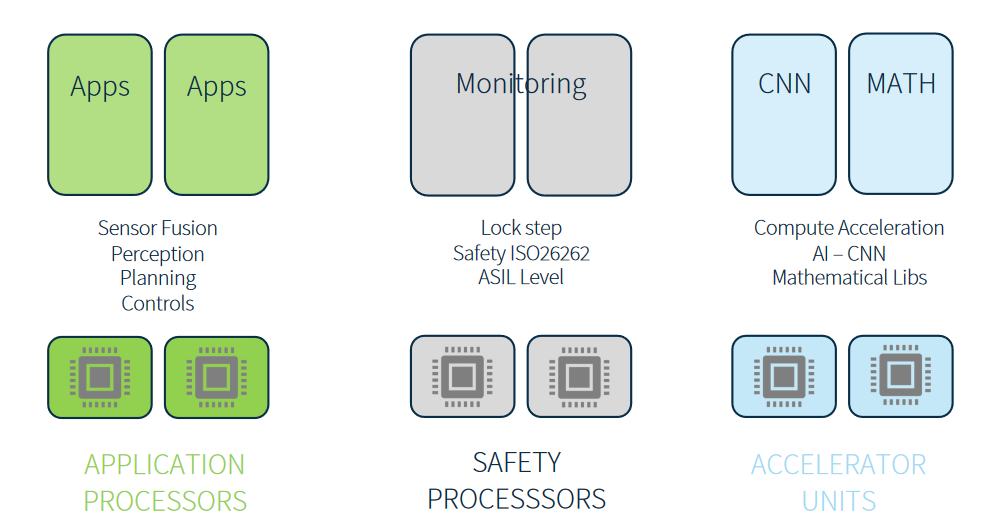
\includegraphics[width=0.6\textwidth]{images/C2_3.png}
    \caption{Processing units in a modern ECU}
\end{figure}

At a high level, we can group the ECUs into three categories, each one mapped to some of the application domains seen above:
\begin{compactitemize}
    \item \textbf{MCU (Microcontroller Unit)}: a small computer on a single integrated circuit chip. Used for airbags, door controls, lighting, climate control, etc. (\textbf{single-core/multi-core}).
          $\Rightarrow$ \textit{Engine control, chassis control, BCMs.}
    \item \textbf{Infotainment (IVI, In-Vehicle Infotainment)}: delivers entertainment and information to driver and passengers through audio/video interfaces (FPGA, GPU, ASIC, multi-core).
          $\Rightarrow$ \textit{Infotainment.}
    \item \textbf{High-end AD/ADAS}: high-performance architectures designed for compute-intensive applications like perception and localization (FPGA, GPU, ASIC, multi-core).
          The trend is a \textbf{heterogeneous design}.
          $\Rightarrow$ \textit{ADAS, AD.}
\end{compactitemize}

\begin{figure}[htbp]
    \centering
    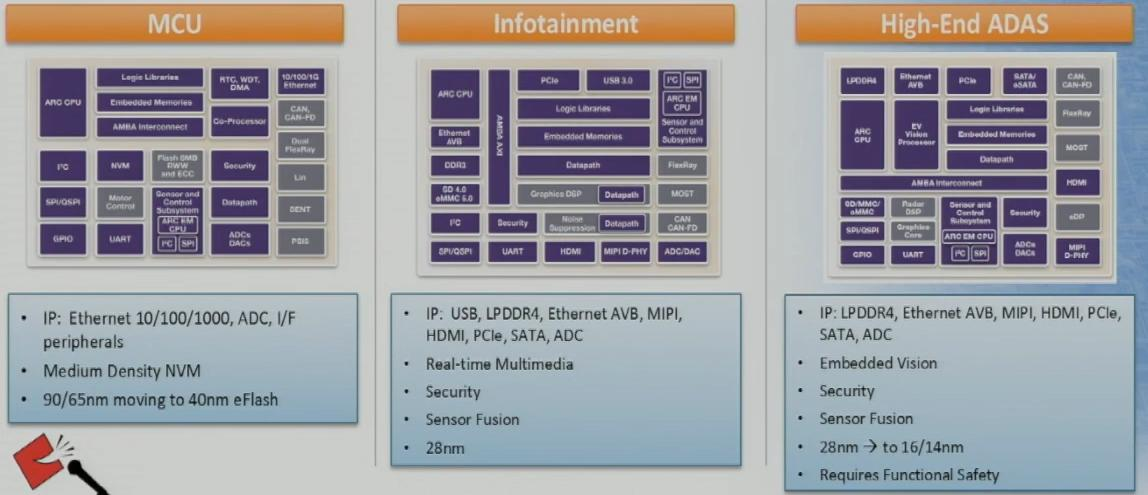
\includegraphics[width=0.8\textwidth]{images/C2_4.png}
    \caption{MCU, Infotainment and High-end ADAS architectures}
\end{figure}

\subsubsection{Microcontroller and microprocessor}
A \textbf{microcontroller} (MCU or $\mu$C) is essentially a \textbf{single chip} that incorporates a microprocessor:
\begin{compactitemize}
    \item it contains one or more CPUs (processor cores) together with \textbf{memory} and programmable \textbf{input/output peripherals};
    \item some microcontrollers execute code directly from the flash memory, so that they can run fast right after powering up;
    \item they are generally used to execute \textbf{small purpose-built programs} in automatically controlled devices, such as engine control systems.
\end{compactitemize}

A \textbf{microprocessor} (MPU) instead is a computer processor that incorporates the functions of a CPU onto just a few integrated circuits, without the memory and the peripherals on the same chip.

\subsection{Computational architectures}
The hardware requirements for processing the car's information can be \textbf{vastly different}: think about the system that controls the car's windows compared to the one that has to understand which objects are in the environment.
For this reason, different computing architectures are used to solve different problems: \textbf{CPU}, \textbf{GPU}, \textbf{FPGA}, \textbf{ASIC}, \dots

Most hardware and software designs consider the \textbf{CPU} as the \textbf{orchestrator}, while the other hardware accelerators are used as \textbf{workers}.

\begin{figure}[H]
    \centering
    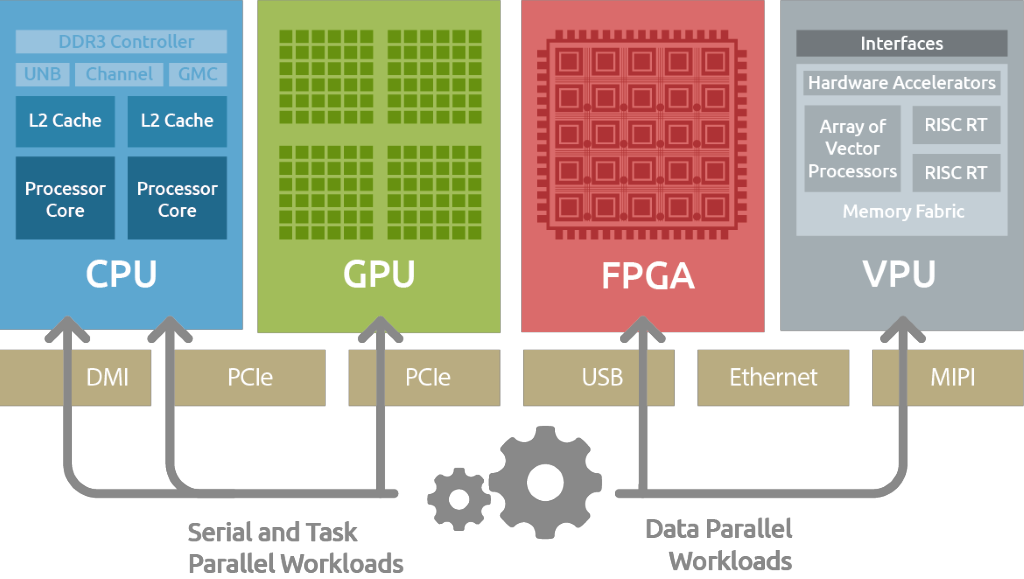
\includegraphics[width=0.65\textwidth]{images/C2_5.png}
    \caption{Computational components: CPU for serial/task-parallel workloads, accelerators for data-parallel workloads}
\end{figure}

\subsubsection{CPU}
The \textbf{CPU} (Central Processing Unit) is the main component of a computer.
A \textbf{single-core} processor is a microprocessor with a single core on a chip, running a \textbf{single thread} at any one time:
\begin{compactitemize}
    \item at the hardware level, the computer executes \textbf{sequences of individual instructions};
    \item each instruction tells the computer to do a simple operation: add, subtract, multiply, etc.
\end{compactitemize}

\subsubsection{From single-core to multi-core}
\begin{wrapfigure}{R}{0.41\textwidth}
    \centering
    \vspace{-10pt}
    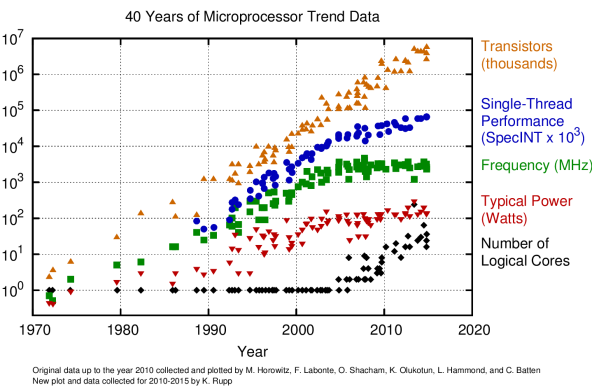
\includegraphics[width=0.4\textwidth]{images/C2_7.png}
    \caption{Microprocessor trend: frequency and power stop growing, the number of cores increases}
    \vspace{-10pt}
\end{wrapfigure}
The shift from single-core to \textbf{multi-core} architectures allowed to integrate more complex software applications.

In the late 1990s and early 2000s the design goal was to \textbf{increase the clock rate}, by adding more transistors to a smaller chip.
Unfortunately, this increased the power dissipation of the chip beyond the capacity of inexpensive cooling techniques: this is known as the \textbf{power wall}.

The \textbf{solution} was to put \textbf{multiple cores on the same die}. Today 4/8 cores are mainstream (and counting), and the same idea of parallelism led to accelerators like GPUs, FPGAs and TPUs.

\subsubsection{GPU}
A \textbf{GPU} (Graphics Processing Unit) is a programmable logic chip originally designed for \textbf{rendering graphics}.

For many critical AD applications, such as pedestrian detection, line following and path planning, the GPU is the \textbf{most popular choice}, since it gives orders of magnitude increases in performance at a modest power consumption.
However:
\begin{compactitemize}
    \item GPUs don't provide as much performance as \textbf{ASICs}, whose hardware is specifically designed for AI (or other) applications;
    \item GPUs deliver a lot of computational power at the expense of \textbf{energy efficiency} and \textbf{heat}.
\end{compactitemize}

The GPU is characterized by the \textbf{host-to-device} paradigm, and the programming language used is \textbf{CUDA}.

\paragraph{GPU hardware model}
\begin{wrapfigure}{R}{0.46\textwidth}
    \centering
    \vspace{-10pt}
    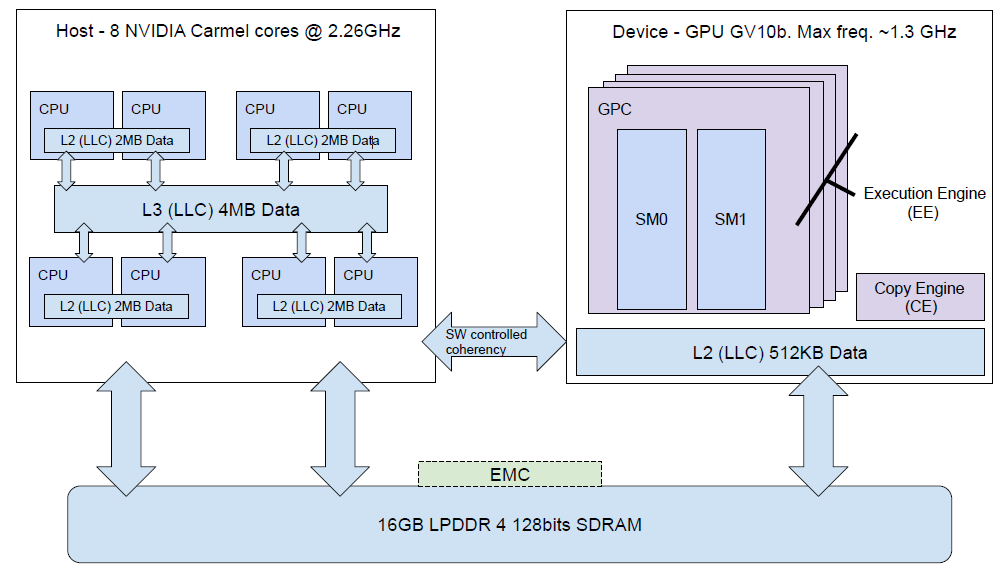
\includegraphics[width=0.45\textwidth]{images/C2_8.png}
    \caption{Heterogeneous CPU-GPU system (host and device)}
    \vspace{-10pt}
\end{wrapfigure}
The typical execution pattern of a heterogeneous CPU-GPU system is:
\begin{enumerate}
    \item move the data from the \textbf{host} (CPU) to the \textbf{device} (GPU);
    \item execute the \textbf{kernel} on the GPU;
    \item move the data from the device back to the host.
\end{enumerate}

The memory copies between host and device are an overhead that has to be taken into account (we will see that this is one of the reasons why Tesla moved away from GPUs).

\subsubsection{FPGA}
An \textbf{FPGA} (Field-Programmable Gate Array) is an integrated circuit designed to be \textbf{configured} by the customer or designer \textbf{after manufacturing}.
It contains an array of \textbf{programmable logic blocks} and a hierarchy of \textbf{reconfigurable interconnects} that allow the blocks to be ``wired together'', like logic gates that can be connected in different configurations.

FPGAs are becoming increasingly important in many domains, where they are used for ``number cruncher'' operations (for example the execution of deep neural networks).

They are programmed using \textbf{hardware description languages} (HDL) such as \textbf{Verilog}, but high-level synthesis tools also allow a subset of C to be compiled into hardware.

\paragraph{FPGA benefits}
\begin{compactitemize}
    \item \textbf{Performance with low latency}: FPGAs provide low latency and also \textbf{deterministic latency}, i.e. a known response time, which is critical for applications with \textbf{hard deadlines}.
    \item \textbf{Cost effectiveness}: FPGAs can be \textbf{reprogrammed} after manufacturing to add functionalities, instead of replacing the hardware.
    \item \textbf{Energy efficiency}: designers can fine-tune the hardware to match the application needs. For example, with \textbf{INT8 quantization} we use 8-bit integers and integer math instead of floating-point numbers and math.
\end{compactitemize}

\subsubsection{ASIC}
An \textbf{ASIC} (Application-Specific Integrated Circuit) is an integrated circuit designed to execute software with a \textbf{specific purpose}: its ALUs and circuits are created only for that task (or set of tasks).
They can contain over two billion transistors (e.g.\ Google's TPU).

ASICs are designed for applications with \textbf{high performance} and \textbf{low power consumption} constraints, but their main drawback is that they are \textbf{not reconfigurable}.
Like FPGAs, they are designed with an HDL such as Verilog or VHDL.

Types of ASICs:
\begin{compactitemize}
    \item \textbf{VPUs} (Vision Processing Units): image/vision processors and co-processors;
    \item \textbf{TPUs} (Tensor Processing Units): focused on specific operations like matrix multiplications, they offer reduced latency and higher energy efficiency (e.g.\ the first TPU developed by Google for TensorFlow);
    \item \textbf{NCUs} (Neural Compute Units), such as the ones from ARM.
\end{compactitemize}

\begin{infobox}[Waymo]
Waymo vehicles are full of sensors: \textbf{LiDAR}, \textbf{cameras}, \textbf{radar} and also \textbf{microphones} (important, e.g.\ to hear sirens).
All these data streams are processed by the \textbf{carTPU}, a purpose-built \textbf{ASIC} that performs the sensor fusion with ultra-low latency, consuming less than 75\,W.
\end{infobox}

\begin{infobox}[Tesla]
Until 2018 (HW2/HW2.5) Tesla ran its neural networks on \textbf{NVIDIA} GPUs (Drive PX2). In 2019, with \textbf{HW3}, it moved to a \textbf{home-made} chip (FSD chip, with dedicated neural network processors). The reasons:
\begin{compactitemize}
    \item \textbf{No CPU-GPU transfers}: camera images go directly to the on-chip memory (SRAM), removing the PCIe copies $\Rightarrow$ lower latency and power;
    \item \textbf{Performance}: chip custom-built for Tesla's neural networks (144 TOPS vs.\ $\sim$8 TOPS of the PX2);
    \item \textbf{Less dependency}: full control of the silicon roadmap and of the costs.
\end{compactitemize}
\end{infobox}

\subsubsection{Comparison}
\begin{table}[H]
    \centering
    \begin{tabular}{|l|c|c|c|c|}
        \hline
         & \textbf{MCU} & \textbf{GPU} & \textbf{FPGA} & \textbf{ASIC} \\
        \hline
        \textbf{Computing power}  & Moderate  & Good/Very good & Good/Very good & Good/Very good \\
        \hline
        \textbf{Programmability}  & Very good & Good           & Not bad        & Poor \\
        \hline
        \textbf{Power efficiency} & Not bad   & Poor           & Good           & Very good \\
        \hline
        \textbf{Flexibility}      & Good      & Very good      & Not bad        & Poor \\
        \hline
    \end{tabular}
    \caption{Pros and cons of the computational architectures (automotive)}
\end{table}

\begin{figure}[H]
    \centering
    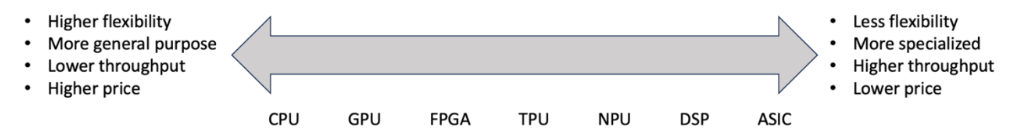
\includegraphics[width=0.75\textwidth]{images/C2_9.png}
    \caption{From general purpose (CPU) to specialized (ASIC) architectures}
\end{figure}

\subsubsection{Silicon war}
When choosing the computing platform, different metrics can be considered:
\begin{compactitemize}
    \item \textbf{Latency}: how long it takes the software to go from the input signal to the decision;
    \item \textbf{Power}: how much electrical energy it takes to make that decision.
\end{compactitemize}

In \textbf{mission-critical systems} the most important property is \textbf{determinism}: we need \textbf{low latency} and \textbf{low jitter} (the difference between the best-case and the worst-case latency), but power consumption is also important.


\begin{infobox}[Not covered in the exam]
The following topics are not part of the exam, but they are interesting:
\begin{compactitemize}
    \item \textbf{Architecture safety}: how we configure CPUs and the other components to guarantee safety.
    \item \textbf{ECU organization}: how we organize the tens/hundreds of ECUs inside a vehicle. \\
          \textit{Spoiler}: today the goal is to \textbf{centralize} the intelligence, not to distribute it.
\end{compactitemize}
\end{infobox}


\subsection{Safety}
\textbf{Safety} is about providing a \textbf{safe answer} while \textbf{handling failures}: a safe system is able to respond correctly even when a problem occurs, trying to \textbf{mitigate} it.

Computers are designed to achieve different goals: high performance, power efficiency, cost, performance/cost and \textbf{safety}.
For safety, two concepts are fundamental:
\begin{compactitemize}
    \item \textbf{Diversity}: using different methods, architectures or technologies to achieve the same function;
    \item \textbf{Redundancy}: duplicating critical components or functions to provide a backup in case of failure.
\end{compactitemize}

The keyword when we talk about safety is only one: \textbf{redundancy}.

\begin{infobox}[Why safety matters]
Most of the incidents involving autonomous vehicles happen because the vehicle is not able to properly detect all the obstacles (e.g.\ cars that suddenly appear).
\end{infobox}

\subsubsection{ISO 26262}
\textbf{ISO 26262} is the adaptation of IEC 61508 to the specific needs of \textbf{electrical/electronic (E/E) systems} in road vehicles. It:
\begin{enumerate}
    \item provides an automotive safety \textbf{lifecycle} (management, development, production, operation, service, decommissioning);
    \item provides an automotive-specific \textbf{risk-based approach} to determine the integrity levels, called \textbf{ASIL} (Automotive Safety Integrity Levels, from A to D);
    \item uses the ASILs to specify the requirements needed to \textbf{avoid unreasonable residual risk};
    \item provides \textbf{requirements for validation} and confirmation, to ensure an acceptable level of safety;
    \item provides requirements for the relations with \textbf{suppliers}.
\end{enumerate}

ISO 26262 does not give strict guidelines, but it provides \textbf{recommendations} for the development of safe hardware and software (e.g.\ how to communicate a hazard, validation requirements, etc.).

\subsubsection{Safe E/E architecture}
How can we guarantee a safe software and hardware deployment? It \textbf{depends on how the hardware has been designed}.
To support the safety requirements of automotive applications, CPUs should provide safe designs, able to:
\begin{compactitemize}
    \item \textbf{detect} their own operational failures in real time and react in a way that avoids harming people;
    \item in case of failure, rely on \textbf{redundancy}, i.e.\ extra components that increase the reliability and availability of the system.
\end{compactitemize}

According to ISO 26262, \textbf{redundancy} is the ``existence of means in addition to the means that would be sufficient for an element to perform a required function or to represent information''.
It can be implemented in:
\begin{compactitemize}
    \item \textbf{Software}: software replication, software diversity, \dots
    \item \textbf{Hardware}: lockstep, asymmetric, symmetric, \dots
\end{compactitemize}

The CPU safety designs can be classified as: \textbf{single core}, \textbf{single core with hardware checking}, \textbf{dual-core lockstep}, \textbf{asymmetric dual core} and \textbf{symmetric dual core}.

\begin{figure}[H]
    \centering
    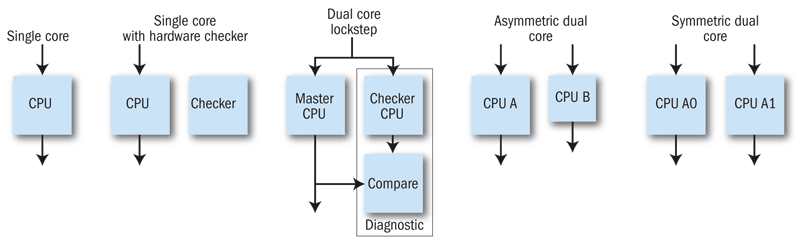
\includegraphics[width=0.6\textwidth]{images/C2_10.png}
    \caption{CPU safety designs}
\end{figure}

\paragraph{Software redundancy (single core)}
\begin{wrapfigure}{R}{0.41\textwidth}
    \centering
    \vspace{-10pt}
    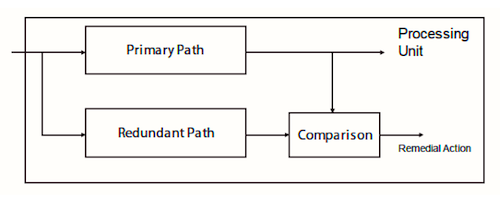
\includegraphics[width=0.4\textwidth]{images/C2_11.png}
    \caption{Software redundancy: primary and redundant path}
    \vspace{-10pt}
\end{wrapfigure}
A single-core processor runs a single thread (or process) at a time, so safety is obtained at the \textbf{software level}, with \textbf{software-based diagnostics}:
\begin{compactitemize}
    \item two software implementations (different or the same) run on the \textbf{same platform}: ideally, one thread spawns two threads that execute the same algorithm, or different algorithms that should produce the same result;
    \item the results of the two paths are \textbf{compared}, and if they differ a remedial action is taken;
    \item \textbf{algorithm diversity}: different algorithms are used for the same task, e.g.\ computing $A+B=C$ versus $C-B=A$.
\end{compactitemize}

\paragraph{Monolithic architecture}
\begin{wrapfigure}{R}{0.41\textwidth}
    \centering
    \vspace{-10pt}
    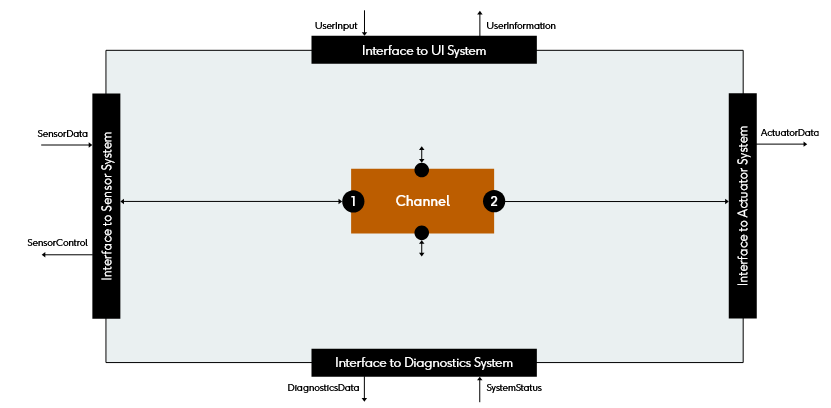
\includegraphics[width=0.4\textwidth]{images/C2_12.png}
    \caption{Monolithic architecture: one single channel between sensors and actuators}
    \vspace{-10pt}
\end{wrapfigure}
The simplest conceptual architecture: \textbf{all the AD tasks} (sensing, perception, planning and control) are performed by a \textbf{single central channel}.
The problem is that a \textbf{single} software bug or hardware fault can lead to unsafe behaviour or to a total system failure (single point of failure).

\paragraph{Hardware redundancy -- Lockstep}
Dual-core \textbf{lockstep} systems are fault-tolerant computers with real \textbf{physical redundancy}: two cores run the \textbf{same set of operations at the same time} (same clock cycle) in parallel.
\begin{compactitemize}
    \item low complexity and widely used;
    \item a \textbf{hardware checker} compares the results: if they are not identical, a fault is assumed to have occurred;
    \item \textbf{no software overhead} to verify the results (the software sees only one core).
\end{compactitemize}

\begin{figure}[H]
    \centering
    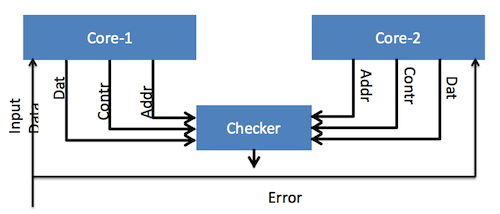
\includegraphics[width=0.4\textwidth]{images/C2_13.png}
    \caption{Dual-core lockstep}
\end{figure}

\paragraph{Hardware redundancy -- Delayed lockstep}
\begin{wrapfigure}{R}{0.39\textwidth}
    \centering
    \vspace{-10pt}
    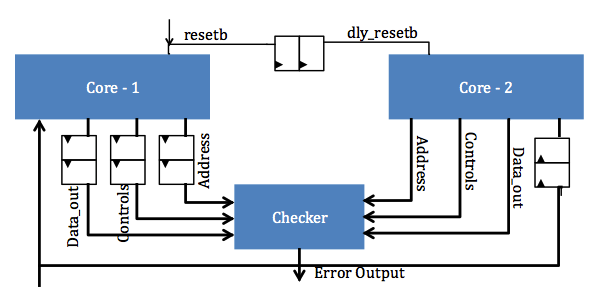
\includegraphics[width=0.38\textwidth]{images/C2_14.png}
    \caption{Delayed lockstep}
    \vspace{-10pt}
\end{wrapfigure}
Like the lockstep, but the \textbf{inputs of one core are delayed by $N$ clock cycles}.
Since the second core performs the same operation $N$ cycles later, the probability that a noise pulse hits both cores affecting them in the same way is much lower: we obtain \textbf{time diversity}.
In some applications having the same clock is not needed; on the contrary, a temporal shift guarantees a different behaviour over time.

\paragraph{Hardware -- Asymmetric design}
\begin{wrapfigure}{R}{0.41\textwidth}
    \centering
    \vspace{-10pt}
    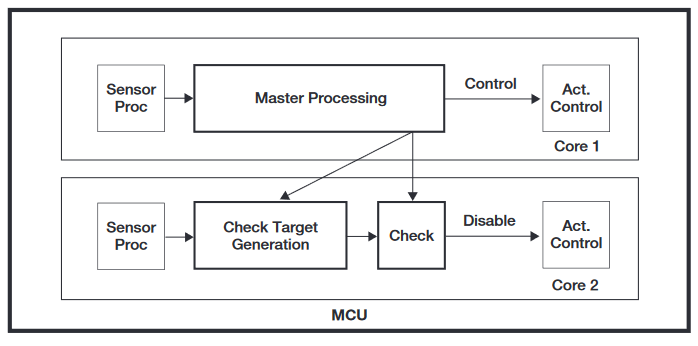
\includegraphics[width=0.4\textwidth]{images/C2_15.png}
    \caption{Asymmetric design: master core and checker core}
    \vspace{-10pt}
\end{wrapfigure}
Two processors with \textbf{different hardware architectures} (typically also running at different frequencies):
\begin{compactitemize}
    \item a separate process checks that the software is working correctly $\Rightarrow$ \textbf{easier to certify};
    \item issues in both CPU and software are easier to detect, thanks to the diverse hardware and software implementations;
    \item the \textbf{performance delta} between the two cores can help or hinder the safety assessment.
\end{compactitemize}

\paragraph{Hardware -- Symmetric design}
Two instances of the software run on two cores with the \textbf{same hardware architecture} and the \textbf{same inputs}:
\begin{compactitemize}
    \item diverse algorithms can also be used (more safety);
    \item results are compared by hardware/software;
    \item unlike lockstep, the cores are \textbf{not synchronized} (in lockstep the software sees only one core, here it sees two);
    \item it follows the \textbf{doer-checker} approach: the \textbf{doer} implements the normal functionality, the \textbf{checker} implements the fail-safe mechanisms.
\end{compactitemize}
\begin{figure}[H]
    \centering
    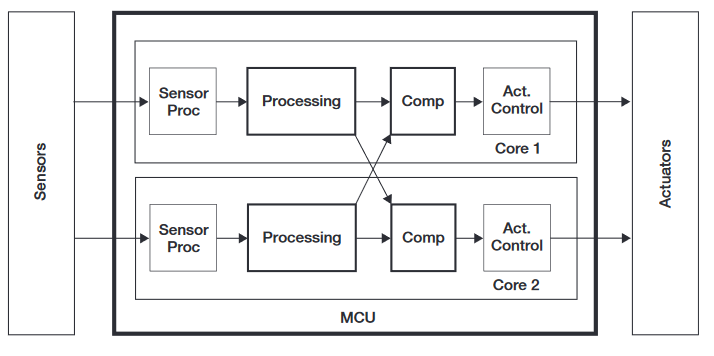
\includegraphics[width=0.4\textwidth]{images/C2_16.png}
    \caption{Symmetric dual-core design}
\end{figure}


\paragraph{Summary}
\begin{table}[H]
    \centering
    \begin{tabular}{|p{4.2cm}|>{\centering\arraybackslash}p{2.6cm}|>{\centering\arraybackslash}p{2.6cm}|>{\centering\arraybackslash}p{2.6cm}|>{\centering\arraybackslash}p{2.6cm}|}
        \hline
         & \textbf{SW complexity} & \textbf{Silicon complexity} & \textbf{Safety analysis complexity} & \textbf{Available performance} \\
        \hline
        \textbf{Single core}                & High   & Low            & High   & Low \\
        \hline
        \textbf{Single core + HW checking}  & Medium & Medium         & Medium & High \\
        \hline
        \textbf{Dual-core lockstep}         & Low    & Medium to high & Low    & High \\
        \hline
        \textbf{Asymmetric dual core}       & Medium to high & Medium to high & Medium & Medium to high \\
        \hline
        \textbf{Symmetric dual core}        & Low    & High           & High   & Medium to high \\
        \hline
    \end{tabular}
    \caption{Comparison of the CPU safety designs}
\end{table}

\subsubsection{Safe AD architectures (state of the art)}
Good, but if we have redundancy and the two cores (or threads) return two different results, \textbf{which one do we trust}?
And what do we do when something goes wrong? We have to choose a \textbf{Minimum Risk Maneuver (MRM)}, and the right one depends on the context: stopping the vehicle can be safe in some situations, but absolutely not in others (e.g.\ in the middle of a highway).

The task is therefore to \textbf{choose a safe trajectory, tolerant to faults}.
All the recent architectures answer the same challenge: an AD system must be \textbf{fail-degraded}, i.e.\ it must tolerate faults and functional insufficiencies of its HW/SW components and keep operating safely for a minimum amount of time, even when something is broken.

They are all variants of the \textbf{Doer/Checker} pattern and they differ in \textbf{how the redundancy is organized}:
\begin{compactitemize}
    \item \textbf{Cross-Checking Pair} $\Rightarrow$ \textbf{symmetric}: 2 channels that validate each other;
    \item \textbf{Daruma} $\Rightarrow$ \textbf{extended symmetric}: 3 channels validated by a dedicated arbiter that picks the best one;
    \item \textbf{AD-EYE} $\Rightarrow$ \textbf{asymmetric}: a high-performance channel supervised by a minimal safety channel, with different, non-interchangeable roles.
\end{compactitemize}
Comparing them allows to evaluate the trade-offs between complexity, cost, robustness, scalability and ease of formal validation.

\paragraph{Doer/Checker pattern}
\begin{compactitemize}
    \item \textbf{Doer}: a \textbf{complex} subsystem that performs the nominal function and generates an output (e.g.\ a trajectory);
    \item \textbf{Checker}: a \textbf{high-integrity, low-complexity} monitor that validates the Doer's output against safety rules;
    \item \textbf{Arbiter (Decider)}: evaluates the Checker's yes/no verdict. If the Checker disapproves or does not respond, the Arbiter \textbf{silences the Doer} to prevent unsafe actions.
\end{compactitemize}
Doer and Checker must be \textbf{independent}, to avoid common cause failures.

\begin{figure}[H]
    \centering
    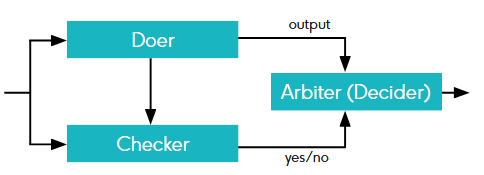
\includegraphics[width=0.4\textwidth]{images/C2_17.png}
    \caption{Doer/Checker pattern}
\end{figure}

\paragraph{Cross-Checking Pair (CCP)}
\noindent
\begin{minipage}[t]{0.62\textwidth}
\vspace{0pt}
\textbf{Symmetric} architecture based on the Doer/Checker pattern, made of \textbf{2 complex channels} and \textbf{2 simple selectors}.
Each channel is at the same time a doer (it produces trajectories) and a checker (it validates the trajectories of the other channel).


How it works:
\end{minipage}\hfill
\begin{minipage}[t]{0.34\textwidth}
\vspace{0pt}
    \centering
    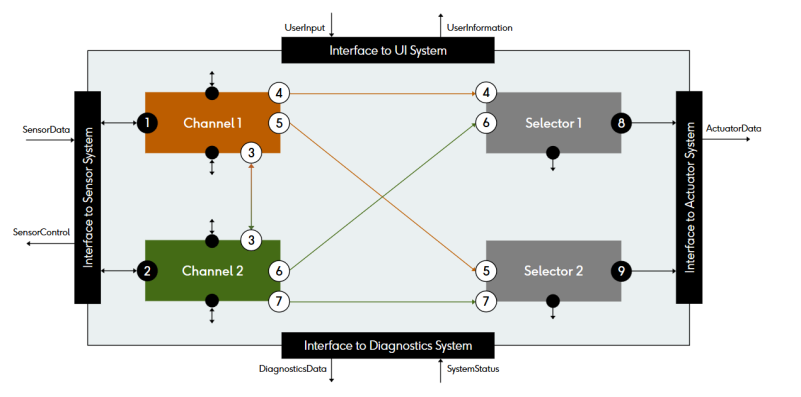
\includegraphics[width=\linewidth]{images/C2_18.png}
    \captionof{figure}{Cross-Checking Pair architecture}
\end{minipage}
\begin{enumerate}
    \item \textbf{Perception}: both channels receive the sensor data and each one builds its \textbf{own world (environment) model}.
    \item \textbf{Generation}: each channel produces two trajectories:
    \begin{compactitemize}
        \item a \textbf{nominal} trajectory: comfortable, reactive to traffic, valid only for a few seconds;
        \item a pre-planned \textbf{MRM} trajectory: valid for the entire maneuver (e.g.\ pulling over).
    \end{compactitemize}
    \item \textbf{Cross-validation}: channel 1 receives the output of channel 2 (and vice versa) and validates it against its \textbf{own} world model, producing an \textbf{OK/NOK} result and a \textbf{score} (comfort, speed, efficiency, e.g.\ smooth trajectories, steering wheel steady most of the time).
    \item \textbf{Sending to the selectors}: each channel sends to both selectors its own commands and the result of the cross-validation.
    \item \textbf{Selector decision} (done separately for the nominal and the MRM trajectories):
    \begin{compactitemize}
        \item if \textbf{both} trajectories are OK for both channels $\Rightarrow$ forward the one with the \textbf{best score};
        \item if \textbf{only one} is OK for both channels $\Rightarrow$ forward that one and \textbf{notify the diagnostics};
        \item if \textbf{none} is OK $\Rightarrow$ no nominal output: the actuator system falls back to the \textbf{buffered MRM}.
    \end{compactitemize}
\end{enumerate}

\paragraph{Daruma}
\begin{wrapfigure}[7]{r}{0.32\textwidth}
    \centering
    \vspace{-10pt}
    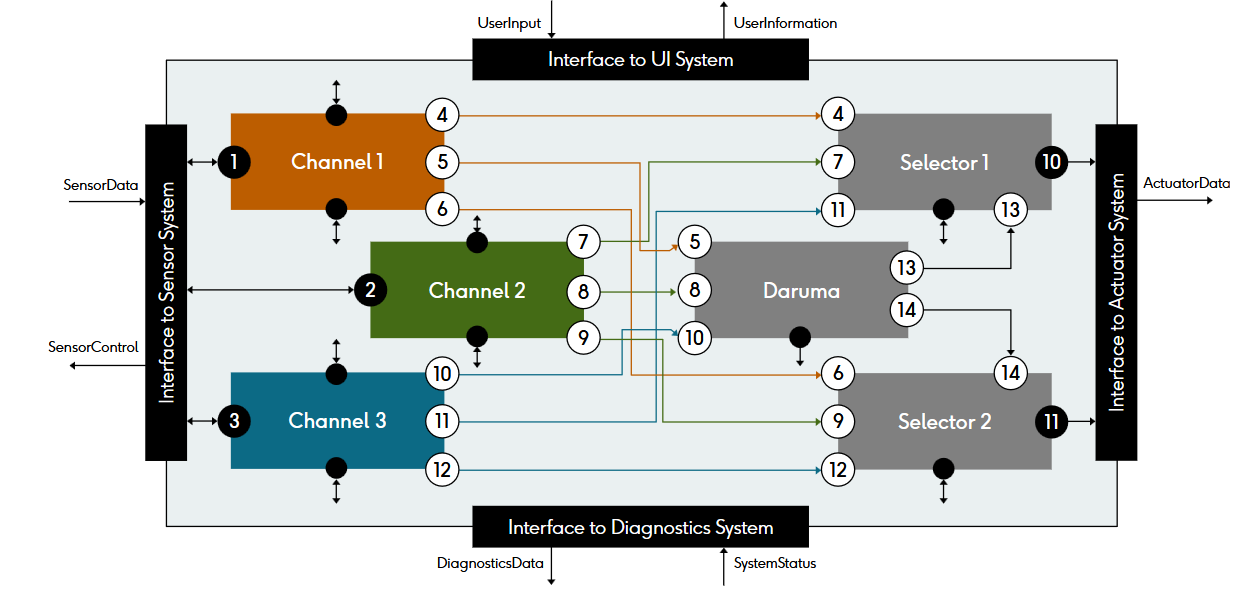
\includegraphics[width=\linewidth]{images/C2_19.png}
    \caption{Daruma architecture}
    \vspace{-10pt}
\end{wrapfigure}
\textbf{Scalable} architecture based on the Doer/Checker pattern, made of \textbf{3 channels}, \textbf{1 Daruma} subsystem and \textbf{2 selectors} (redundant, for fault tolerance).
The key difference with CCP is that the validation is done by a dedicated subsystem, the \textbf{Daruma}, which prefers the trajectory with the \textbf{best evaluation}, not the one most ``similar to the others'' (as a majority voting would do): in this way the \textbf{diversity} of the channels is better exploited.


How it works:
\begin{enumerate}
    \item \textbf{Perception and generation}: each of the 3 channels independently produces its trajectory (nominal + MRM) and its own world model, and sends everything to the Daruma.
    \item \textbf{$3\times3$ cross-validation}: the Daruma compares \textbf{every trajectory against every world model} (9 comparisons), giving each one a score on:
    \begin{compactitemize}
        \item \textbf{correctness} (no collisions, physical feasibility) $\Rightarrow$ the priority criterion;
        \item comfort, speed, efficiency;
        \item consistency between the world models.
    \end{compactitemize}
    \item \textbf{Ranking}: based on the scores, the Daruma ranks the three channels (e.g.\ Ch1 $>$ Ch2 $>$ Ch3).
    \item \textbf{Sending to the selectors}: the Daruma sends the ranking to the two selectors.
    \item \textbf{Selector decision}: the commands of the \textbf{highest-ranked channel} are forwarded to the actuators; if no channel is safe enough, the \textbf{buffered MRM} is used.
\end{enumerate}

Fault handling:
\begin{compactitemize}
    \item if a \textbf{channel} fails $\Rightarrow$ it is automatically moved down in the ranking, and the other two keep working;
    \item if the \textbf{Daruma itself} fails $\Rightarrow$ the selectors directly switch to the buffered MRM (\textbf{fail-safe}).
\end{compactitemize}

\begin{table}[H]
    \centering
    \begin{tabular}{|l|p{6cm}|p{6cm}|}
        \hline
         & \textbf{Cross-Checking Pair} & \textbf{Daruma} \\
        \hline
        \textbf{Structure}  & 2 channels + 2 selectors & 3 channels + 1 Daruma + 2 selectors \\
        \hline
        \textbf{Validation} & each channel validates the other one & the Daruma validates every trajectory against every world model \\
        \hline
        \textbf{Decision}   & best score among the trajectories OK for both channels & highest-ranked channel \\
        \hline
        \textbf{Fallback}   & buffered MRM & buffered MRM (also if the Daruma fails) \\
        \hline
    \end{tabular}
    \caption{CCP vs Daruma}
\end{table}

\subsection{ECU organizations}
Today cars are designed around a \textbf{domain-oriented approach}: we have an \textbf{ECU that provides a service}, and the ECU is wired to the module (like the engine) or to the sensor.
The main domains are: \textbf{powertrain}, \textbf{chassis}, \textbf{safety}, \textbf{driver assistance/autonomy} and \textbf{cockpit}.

This scales well only if the ECU is \textbf{close to the module}.
The problem is that we have many ECUs, and their number grows with each generation: they cannot all be integrated close to their modules, and wiring all of them makes the \textbf{cabling expensive} and the whole organization complex.
Moreover, the software is often fine-grained legacy code shared between the OEM and the Tier-1, with many dependencies.

So a \textbf{good ECU organization is needed}. The idea that is being followed is to move towards \textbf{few, powerful domain/zonal computers}, instead of many ECUs that take care of tiny functions.

Each domain has very different requirements:

\begin{figure}[H]
    \centering
    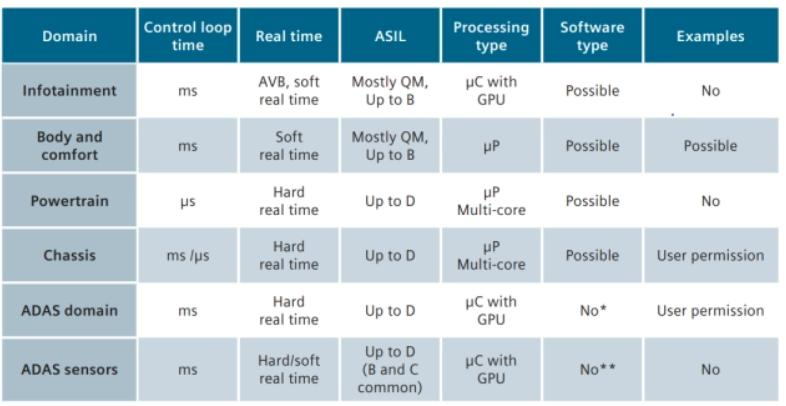
\includegraphics[width=0.7\textwidth]{images/C2_21.png}
    \caption{Requirements of the different vehicle domains}
\end{figure}

\subsubsection{Automotive architectures}
From the OEM point of view it is still unclear which is the most convenient approach for ADAS and self-driving applications, and companies like Bosch, Ford or General Motors are evaluating different paradigms.
The automotive E/E architectures evolved from single decentralized ECUs to an ever-increasing number of ECUs and a closer integration. The three main models are:
\begin{compactitemize}
    \item \textbf{Distributed E/E architecture} (yesterday);
    \item \textbf{Domain centralized E/E architecture} (today);
    \item \textbf{Zonal centralized E/E architecture} (tomorrow).
\end{compactitemize}

\begin{infobox}[The room metaphor]
If the car was a room and the ECUs were people discussing different topics, a domain architecture is like arranging those people chaotically, forcing them to \textbf{shout} across the room to reach the others in their discussion group.
\end{infobox}

\subsubsection{Distributed E/E architecture}
It is the \textbf{most common} automotive architecture: essentially, \textbf{each function} of the vehicle is delivered by a \textbf{specific ECU}.
The ECUs are connected through a \textbf{broadcast bus} (typically CAN bus, but also LIN, FlexRay or automotive Ethernet).

The architecture is \textbf{highly modular}: each ECU is connected to the vehicle network and has an embedded microcontroller that controls its sensors and actuators.

\begin{wrapfigure}{R}{0.27\textwidth}
    \centering
    \vspace{-10pt}
    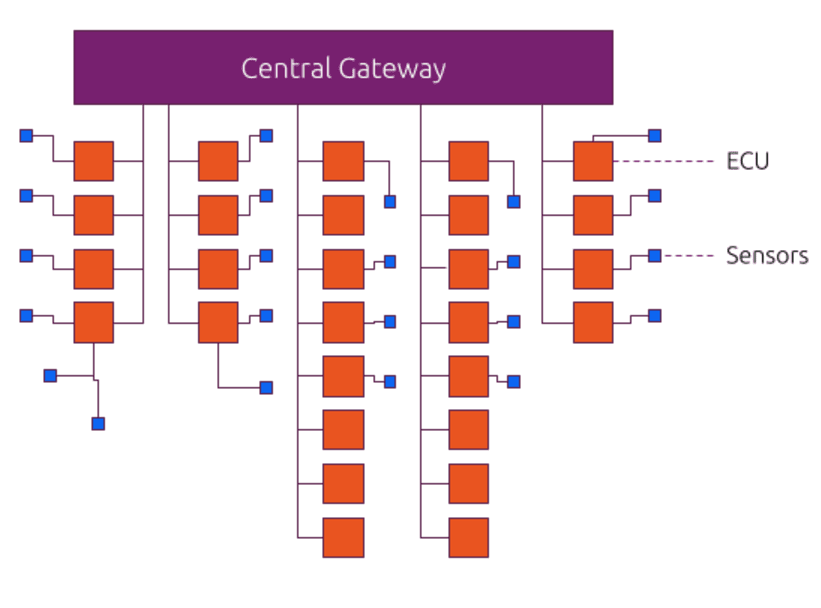
\includegraphics[width=0.26\textwidth]{images/C2_22.png}
    \caption{Distributed E/E}
    \vspace{-25pt}
\end{wrapfigure}
The main drawback is that the OEMs are \textbf{highly dependent on the Tier-1} suppliers (companies like Bosch) for both hardware and software (\textbf{vendor lock-in}): to implement any new function, the OEM needs to call the Tier-1.
This is changing, since OEMs are developing more and more in-house.

Examples: Volvo P80, Ford EUCD, Volkswagen Group B platforms.

\subsubsection{Domain architecture}
\begin{wrapfigure}{R}{0.41\textwidth}
    \centering
    \vspace{-10pt}
    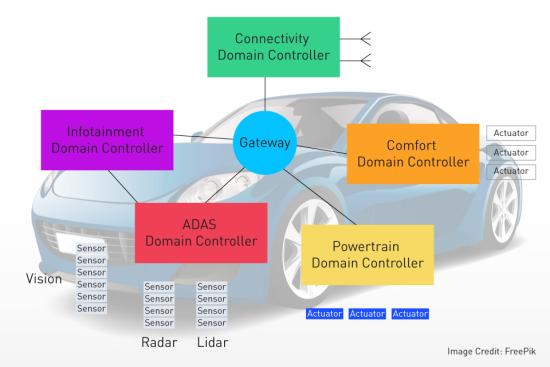
\includegraphics[width=0.4\textwidth]{images/C2_23.png}
    \caption{Domain architecture}
    \vspace{-10pt}
\end{wrapfigure}
The distributed architecture has reached its \textbf{computational limits}.
In the \textbf{domain architecture} the ECUs are grouped by \textbf{domains} (chassis, powertrain, ADAS, infotainment, \dots), and each group is managed by a \textbf{domain controller}.
ECUs can directly communicate only with the ECUs of the same domain, while the different domains are connected through a \textbf{central gateway}.

It focuses on properties such as \textbf{scalability}, \textbf{robustness} and \textbf{maintainability}.

However, all the ECUs are connected to their domain controller, but this does \textbf{not} mean that they are physically \textbf{close} to it.
It scales well only if devices and sensors remain close to the module: for example, an application that reads the temperature of the wheels should be deployed on an ECU close to the wheels. If the ECU that executes it is far away, we have a lot of wiring.

Example: Volvo XC90.

\subsubsection{Zonal architecture}
\begin{wrapfigure}{R}{0.41\textwidth}
    \centering
    \vspace{-10pt}
    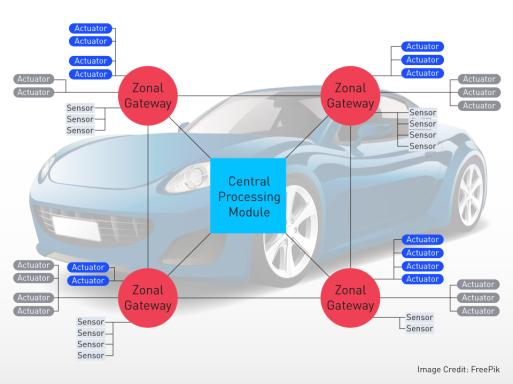
\includegraphics[width=0.4\textwidth]{images/C2_24.png}
    \caption{Zonal architecture}
    \vspace{-10pt}
\end{wrapfigure}
The zonal (or centralized) architecture was introduced to solve the problems of the domain one.
The idea is to \textbf{reduce the number of ECUs} and use only a few very powerful vehicle computers instead of many individual control units:
the ECUs that are \textbf{physically close} are combined under a single \textbf{zonal controller} (zonal gateway), regardless of their domain.

Instead of domains, it uses a \textbf{layered architecture}, and it exploits AI, neural networks, cloud and \textbf{software over-the-air (SOTA)} updates.
A \textbf{high-performance server} (HPC, one or many) acts as the \textbf{brain} of the vehicle. There are two variants:
\begin{compactitemize}
    \item \textbf{Zonal distributed}: multiple HPCs manage the vehicle functionalities (intermediate step);
    \item \textbf{Zonal centralized/consolidated}: a single HPC acts as the master and processes all the data coming from the different zones (we try to centralize as much as possible).
\end{compactitemize}

\begin{figure}[H]
    \centering
    \begin{subfigure}{0.45\textwidth}
        \centering
        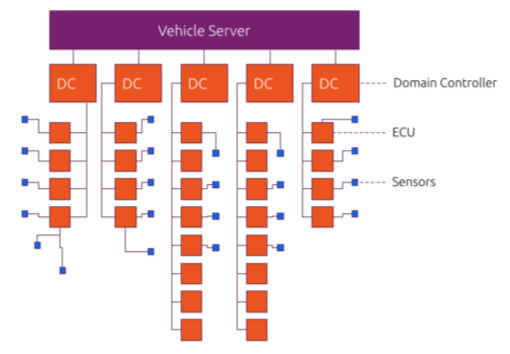
\includegraphics[width=0.8\textwidth]{images/C2_25.png}
        \caption{Zonal distributed}
    \end{subfigure}
    \begin{subfigure}{0.45\textwidth}
        \centering
        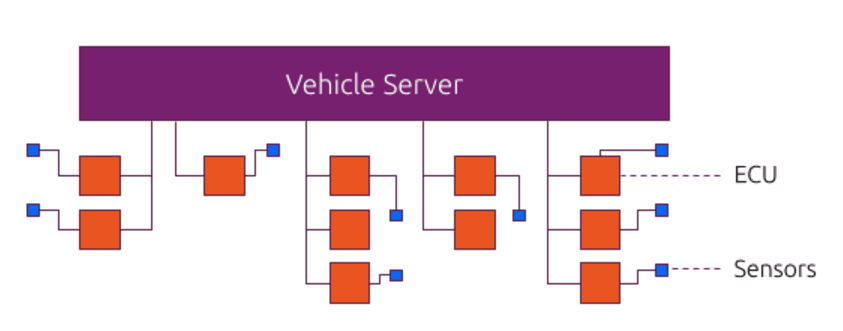
\includegraphics[width=0.8\textwidth]{images/C2_26.png}
        \caption{Zonal centralized}
    \end{subfigure}
    \caption{From domain to zonal architecture}
\end{figure}

The main advantages are:
\begin{compactitemize}
    \item \textbf{Fewer cables}: savings of 50\% and more in the length of the wiring harness. For example, Delphi reported a 30\% saving in wiring mass and cost by centralizing the ADAS features on the Audi A3, and Bosch a 15--20\% reduction in wiring weight going from a domain-oriented to a zone-oriented architecture;
    \item \textbf{Power efficiency};
    \item the savings \textbf{increase} with the number of sensors and actuators.
\end{compactitemize}
Examples: BMW, Volvo cars (SPA2).

\begin{figure}[H]
    \centering
    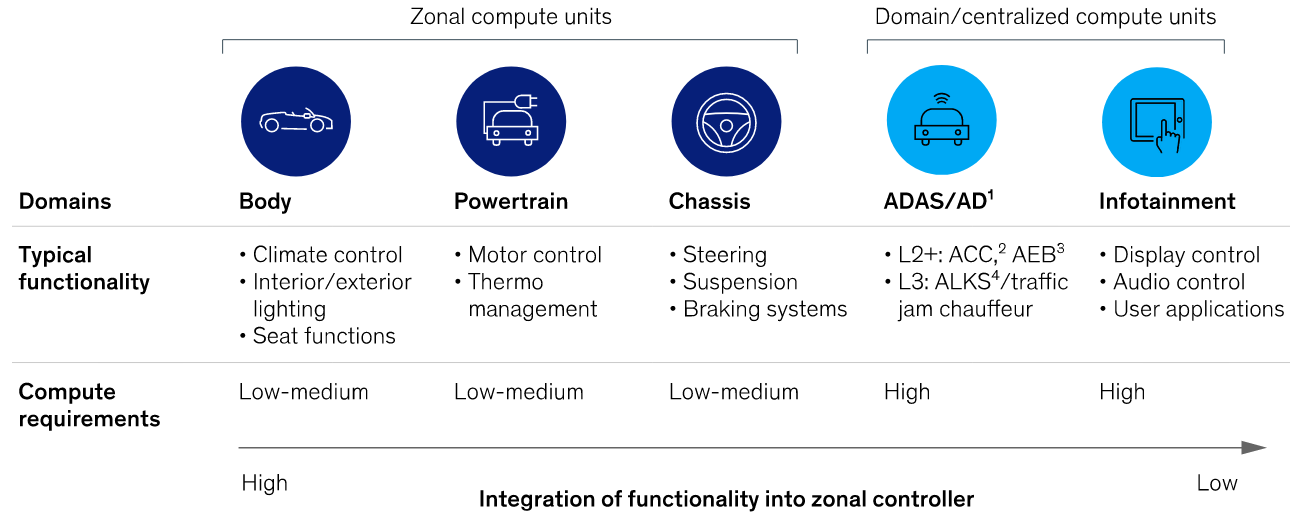
\includegraphics[width=0.65\textwidth]{images/C2_27.png}
    \caption{Which functions are integrated into zonal controllers and which into central compute units}
\end{figure}

\begin{infobox}[Cost matters]
Saving even a hundred euros per car on cables (or on other components) is a huge amount at production scale: this is why some European companies are buying Chinese zonal architectures, to save as much as possible.
\end{infobox}

\subsection{Case studies}

In questa sezione vedremo diversi casi studio.

\subsubsection{Hipert car - Maserati Quattroporte}


\subsubsection{State of the art}
Vedremo ora i setup dei due stati dell'arte che sono \textbf{waymo} e \textbf{tesla}.

\paragraph{Tesla}
Nella tabella di fianco riportata si puo vedere tutta l'evoluzione dei sensori e dell'hw di tesla.
Si può vedere che inizialmente si aveva uno stack vario, con camere ma anche con radar e sensori ultrasuoni, ora invece è completamente passata ad un full camera setup.

\paragraph{Waymo}
Nella tabella di fianco si può vedere tutta l'evelouzione dei sensori e dell'hw du waymo.

Nella tabella sotto si può vedere come le sole camere o i solo LIDAR non permettono grandi perfirmance nella object detection.
Questo va contro le affermazioni di musk e karapthy. Ovviamente tesla internamente probabilemnte raggiunge performance ben maggiori ma comunque le telecamenre hanno limiti indiscutibili.

\paragraph{Truck Hipert}
Ha lidar anche dietro.
Tutto il sistema produce 60Mbit al secondo che in qualche modo va gestito.

\paragraph{Tensor e Cruise}
Allora purtorppo waymo ha un death count di gatti molto alti. Questo perchè non rileva ostacoli sotto il veicolo.
Tensor risolve questo problema.

Incidente che ha fatto fallire Cruise, perchè non avevano sensori sotto il veicolo. 

Per parlare di questo abbiamo bisogno del concetto precedentemente introdotto di ODD, quindi dobbiamo sapere dove il veicolo andrò a guidare.
